%!TEX root = main.tex

\subsection{Rule-based approach}

Use a large dictionary to assign each word a set of possible tags. Apply a large list of disambiguation rules to restrict each set to a single tag for each word. The constraints are used in a negative way, to eliminate the tags that are inconsistent with the context.

\begin{figure}[htp]
	\centering
	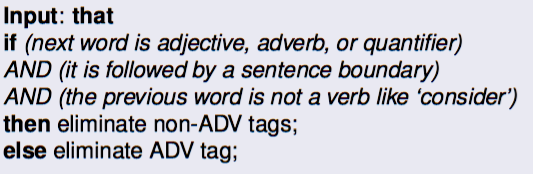
\includegraphics[scale=0.4]{images/35_rules.png}
 	\caption{Example of rules.}
\end{figure}

There are some limitations:
\begin{itemize}
	\item Specific to a given language;
	\item Linguistics ressource need to be updated. 
\end{itemize}

\subsection{Probabilistic approach}

See previous chapter.

\subsection{Transformation-based tagging}

\begin{figure}[htp]
	\centering
	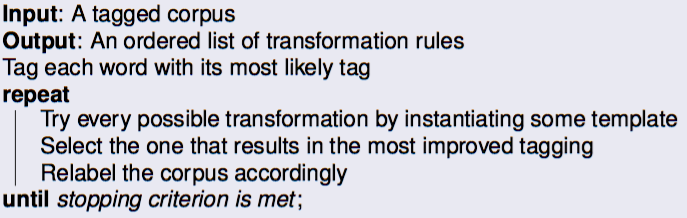
\includegraphics[scale=0.4]{images/36_brill.png}
 	\caption{Brill tagger.}
\end{figure}
 The algorithm need transformations templates (Change tag from \textbf{a} to \textbf{b} when word before is tagged \textbf{z}, \dots) and a tagged corpus. A stopping criterion could be: insufficient improvement over the previous pass. To know if the transformation give a better tagging, the algorithm need a tagged corpus. The output of the TBL process is an ordered list of transformations; these then constitute a tagging procedure that can be applied to a new corpus. 

  \subsubsection{Pros}
  \begin{itemize}
  	\item Transformations rules can be interpreted linguistically;
  	\item Learning those rules makes it possible to adapt the tagger to several languages.
  \end{itemize}
  \subsubsection{Limitations}
  \begin{itemize}
  	\item A transformation rule can be learned only if it is an instance of an abstract transformation template;
  	\item Supervised only, need a tagged corpus;
  	\item Computational complexity of learning is an issue.
  \end{itemize}

\subsection{HMM POS tagging}

\subsubsection{Supervised learning}

\begin{figure}[H]
	\centering
	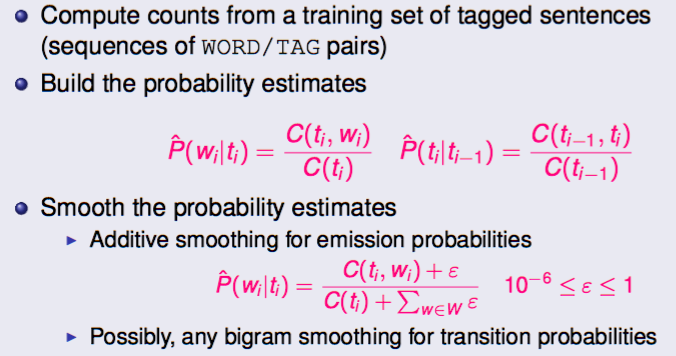
\includegraphics[scale=0.5]{images/38_supervised.png}
 	\caption{HMM tagging = Viterbi decoding.}
\end{figure}

\paragraph{Pro}

We can interpret the states as true POS tag and there is no need to discover the meaning of the states after learning.

\paragraph{Limitations}

A tagged corpus is required.

\subsubsection{Unsupervised learning}
\begin{figure}[H]
	\centering
	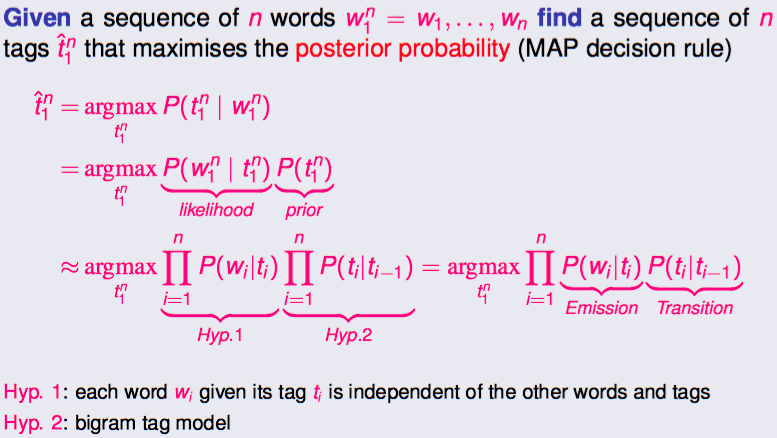
\includegraphics[scale=0.45]{images/37_viterbi.png}
 	\caption{HMM tagging = Viterbi decoding.}
\end{figure}
\paragraph{Pro}

Fully automatic. Define a HMM structure with one state per tag in a tagset and learn the HMM parameters $P(w_i|t_i)$ and $P(t_i|t_{i−1})$ using Viterbi training or Baum-Welch on a text corpus (not tagged!).

\paragraph{Limitations}

Viterbi training and Baum-Welch are sensitive to the initialization. The states are not necessarily associated with relevant tag set, some linguistically informed post-processing needs to be done if one wants to map states to actual tags, whenever possible.

\subsubsection{Notes}

A \textbf{out-of-vocabulary} word in the test set is assigned as a zero probability, there is no Viterbi path. The usual solution is to replace any word occuring only once in the training set with the marker \textit{UNK}. We then need to reduce the observed vocabulary and add \textit{UNK} to it and smooth the emission probability.\\

It is possible to extend HMM to tag trigrams.

\begin{figure}[H]
	\centering
	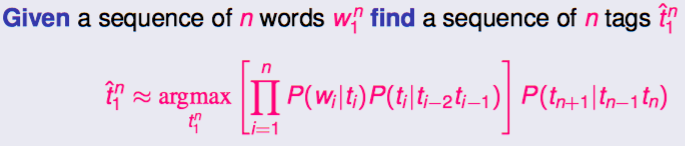
\includegraphics[scale=0.5]{images/39_trigrams.png}
 	\caption{Need to apply n-gram smoothing techniques.}
\end{figure}

\subsection{Evaluation}

\begin{figure}[H]
\centering
\begin{minipage}{.5\textwidth}
  \centering
  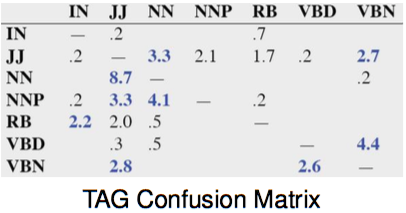
\includegraphics[scale=0.5]{images/40_matrix.png}
\end{minipage}%
\begin{minipage}{.5\textwidth}
  \centering
  \begin{itemize}
  	\item Row is an actual tag;
  	\item Column is predicted tag;
  	\item Entry is error percentage.
  \end{itemize}
\end{minipage}
\end{figure}

There is the formula to assess the perfomance of the tagging.

\begin{itemize}
	\item \textbf{Average error rate per TAG} = $\frac{1}{\# of rows}*\sum_i (\text{total of row i})$;
	\item \textbf{Tagging error rate} = $\frac{\sum_i f(i)*(\text{total of row i})}{\sum_i f(i)}$;
	\item \textbf{Tagging accuracy} = $100\% - \text{Tagging error rate}$.
\end{itemize}